De geleverde grondplannen kwamen over het algemeen overeen met de realiteit, de
enige uitzondering hier op was het grondplan van proefpersoon 17, zijn kaart was
gespiegeld over de as die met de gang mee loopt.

\begin{figure}[h!]
    \centering
    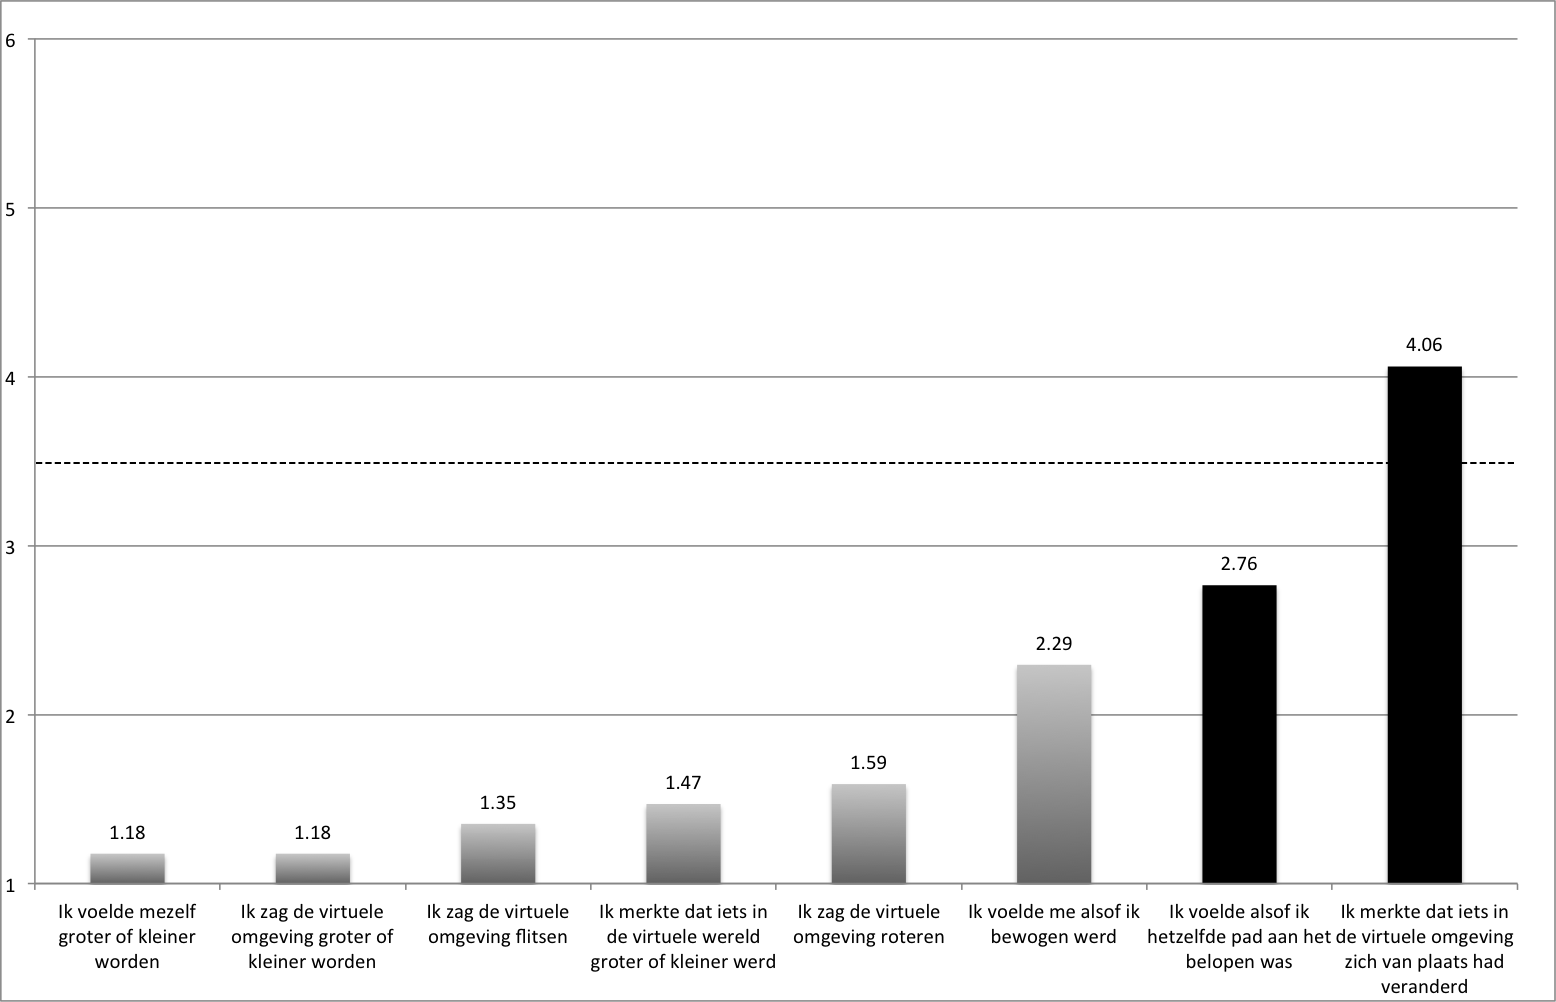
\includegraphics[width=\textwidth]{chart}
    \caption{Grafiek van de gemiddelde scores van de stellingen, de zwarte 
    kolommen zijn de ware stellingen.}
    \label{fig:chart}
\end{figure}

Scores voor de afleidingsstellingen vari\"eren tussen 1.18 en 2.29, de hoge score
van ``Ik voelde me alsof ik bewogen werd'' valt hier op. Vermoedelijk werd die
vraag door sommigen verkeerd ge\"interpreteerd. Zowel ``Ik voelde alsof ik 
hetzelfde pad aan het belopen was'' ($\bar{x}$: 2.76) als ``Ik merkte dat iets in
de omgeving zich van plaats had veranderd'' ($\bar{x}$: 4.06) behaalden zeer hoge
gemiddelde scores. Dit duidt aan dat de verplaatsing van de deur eerder wel
merkbaar was, maar dat de aard van het pad door de fysieke omgeving niet zeer
merkbaar was.

De antwoorden op de vraag waar gevraagd werd het bewogen object te identificeren
duiden aan dat 53\% van de testgroep de verplaatsing van de deuren niet merkte.
Indien ik de scores van de personen die het bewegen van de deur niet correct 
konden identificeren negeer, verlaagt het gemiddelde van de stelling ``Ik merkte 
dat iets in de omgeving zich van plaats had veranderd'' naar $\bar{x}$: 3.18.
Deze waarde zou aanduiden dat het verplaatsen eerder niet merkbaar was.

Verder wil ik opmerken dat geen enkele proefpersoon een opmerking heeft gemaakt
over de snelheidsschalering van 110\%. Hier werd echter niet voor getest, want ik
ben er van uit gegaan dat deze waarde onmerkbaar is wegens de resultaten van
Steinicke et. al., 2009 \cite{steinicke09}.


\section{Bespreking feedback}
Een van de vragen op de vragenlijst vroeg of er iets was dat de immersie breekt.
Er werd hier feedback gegeven op diverse problemen:

\begin{itemize}
  \item Fysieke problemen zoals de grootte van de Oculus Rift, het storen van de
        kabels, en rakelings tegen het doek lopen.
  \item Technische problemen zoals het ontbreken van een realistisch input device
        en de resolutie van de Oculus Rift.
\end{itemize}

Als laatste heb ik ook feedback gekregen dat er kleine haperingen in de tracking
waren, helaas zijn deze kleine haperingen veroorzaakt door een onvoldoende aantal
cameras en kon ik hier niets aan doen. Wegens een kleine hoeveelheid 
netwerklatency zat er ook een beetje lag op de reactiesnelheid van het systeem. 
Een van de proefpersonen was ook te groot voor de tracking setup en moest een
beetje gebukt door de omgeving lopen. Enkele van de proefpersonen die de 
verplaatsing van de deur merkten noteerden dit ook als immersiebrekend.